% \documentclass[handout]{beamer}
\documentclass[]{beamer}
    \usetheme{Boadilla}
    \usecolortheme{beaver}

% \usepackage[fleqn]{amsmath}
\usepackage[italicdiff]{physics}
\usepackage{siunitx}
\usepackage{amssymb,xparse}
	\usepackage[makeroom]{cancel} %% \cancelto{value}{expression}
\usepackage{caption}
\usepackage{subcaption}

\usepackage{graphicx}

\usepackage{dutchcal}  %changes \mathcal, \mathbcal for script r (E&M)
\newcommand{\Letter}[1]{\mathcal{#1}}
\newcommand{\Lag}{\Letter{L}}
\newcommand{\Sl}{\ell} % Lowercase script l 
\newcommand{\Def}{\equiv}
\newcommand{\goesto}{\quad\Rightarrow\quad}
\newcommand{\prop}{\propto}
\newcommand{\p}{\partial}

\title[Analysis of Equations of State]{Analysis of Equations of State for Neutron Star Modeling}
\author{Joseph Nyhan}
\date{April 27, 2022}
\institute{College of the Holy Cross}

\begin{document}

    \maketitle

    \begin{frame}{Outline}
        \pause
        \begin{itemize}
            \item What is a neutron star? \pause
            \item What is an equation of state (EoS)? \pause How do they fit into our model of a neutron star? \pause
            \item How can we use an EoS to make macroscopic predictions about neutron stars? \pause
            \item An example and its predictions: \pause
            \begin{itemize}
                \item QHD-I
            \end{itemize}
        \end{itemize}
    \end{frame}

    \begin{frame}{Neutron Stars}
        \pause
        \begin{itemize}
            \item The collapsed core of a supergiant star \pause
            \item After a supernovae explosion, the dense core is left over \pause
            \item Radius: $\sim\SI{10}{km}$\pause ; Mass: $\sim\SI{1}{\odot}$. \pause
            \item Made mostly of neutrons, protons, and electrons\pause ; overall, is neutral \pause
            \item Core held together by intense gravitational attraction \pause
            \begin{itemize}
                \item Gravitational acceleration on Earth's Surface: $\approx \SI{10}{m/s^2}$ \pause
                \item Neutron star: $\approx \SI{e12}{m/s^2}$ \pause (escape velocity $\sim \SI{100000}{km/s} = $ \pause $c/3$)\pause
            \end{itemize}
            \item Why are they interesting? \pause \begin{itemize}
                \item Smallest, densest observed stellar objects \pause
                \item Exotic physics
            \end{itemize}
        \end{itemize}
    \end{frame}

    \begin{frame}{Equation of State (EoS)}
        What is an equation of state? \pause
        \begin{itemize}
            \item A relationship between \textit{energy density} (denoted $\epsilon$) \pause and pressure (denoted $P$) \pause \begin{itemize}
                \item $\epsilon = \epsilon (P)$\pause $~~ \Leftrightarrow ~~  P = P(\epsilon)$ \pause
            \end{itemize}
            \item Encodes the fundamental interparticle interactions within a neutron star \pause
            \item True EoS within a neutron star is unknown; \pause multitude of candidates, each based on a slightly different model \pause \begin{itemize}
                \item Models can be very complicated\pause ; often simplifications must be made \pause
            \end{itemize}
        \end{itemize}
    \end{frame}

    % \begin{frame}{Using an Equation of State to Make Predictions}
    %     \begin{itemize}
    %         \item TOV equations \pause
    %         \item Mass rad
    %     \end{itemize}
    % \end{frame}

    % \begin{frame}{The Tolman-Oppenheimer-Volkoff (TOV) Equations}
    %     \pause Used to describe a static (time independent) spherically symmetric neutron star. \pause Given by
    %     \begin{align*}
    %         \dv{m}{r} = 4\pi r^2 \epsilon, \quad \dv{P}{r} = -\frac{(4\pi r^3 P + m)(\epsilon + P)}{r^2 (1-2m/r)}.
    %     \end{align*}
    %     where $\epsilon$ is energy density, $P$ is pressure, and $m$ is mass. \pause Use EoS to determine $\epsilon~$\pause $=\epsilon(P)$. \pause Initial conditions: \pause
    %     \[m(r=0) = 0, \quad P(r=0) \Def P_0 = \text{const.}\]\pause
    %     Each solution uniquely specified by $P_0$. \pause Outer conditions: \pause \textit{radius} of the star, $R$\pause , and \textit{mass} of the star, $M$\pause , defined by \[P(R) = 0, \quad M = m(R).\] \pause
    %     Solve an \textit{initial value problem}. \pause A solution to the above system is called a \textit{static solution}.         % \begin{itemize}
    %     %     \item System of two coupled ordinary differential equations (ODEs) \pause
    %     %     \item Solve using a numerical integration technique \pause
    %     %     \item Solution called a ``static solution''
    %     % \end{itemize}
    % \end{frame}

    \begin{frame}{Static Solutions}
        \pause
        \begin{itemize}
            \item Solve a system of equations to produce an ``image'' of a neutron star \pause
            \begin{itemize}
                \item Called the Tolman-Oppenheimer-Volkoff (TOV) equations \pause
            \end{itemize}
            \item Specify an EoS and a \textit{central pressure} $P_0$ and get curves describing $\epsilon$, $P$, and $m$. \pause 
            \item A solution is known as a \textit{static solution}\pause ; spherically symmetric\pause
        \end{itemize}

        \begin{figure}[h!]
            \centering
            \begin{subfigure}{.5\textwidth}
                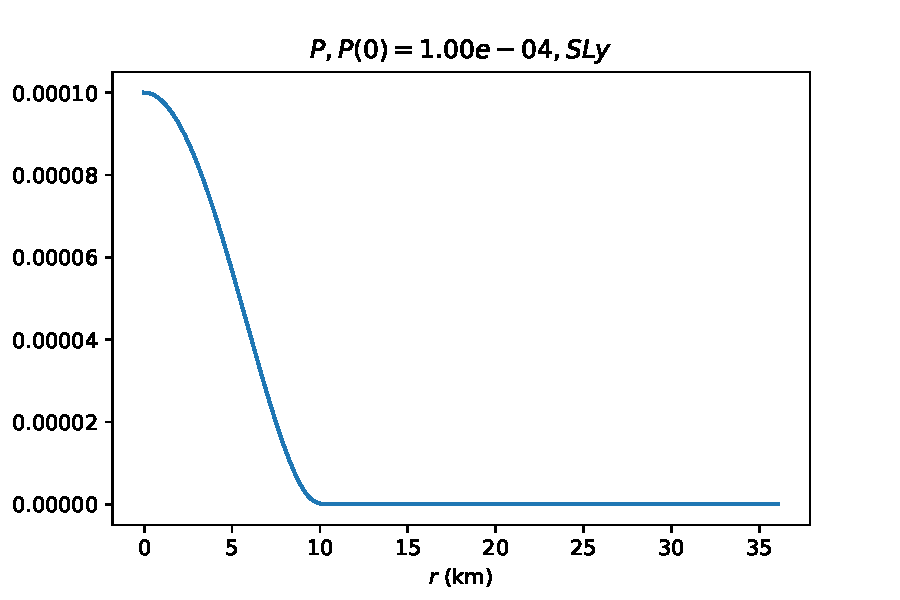
\includegraphics[width = \textwidth]{../paper/images/tov/SLy_P,p00.0001.pdf}
            \end{subfigure}%
            \begin{subfigure}{.5\textwidth}
                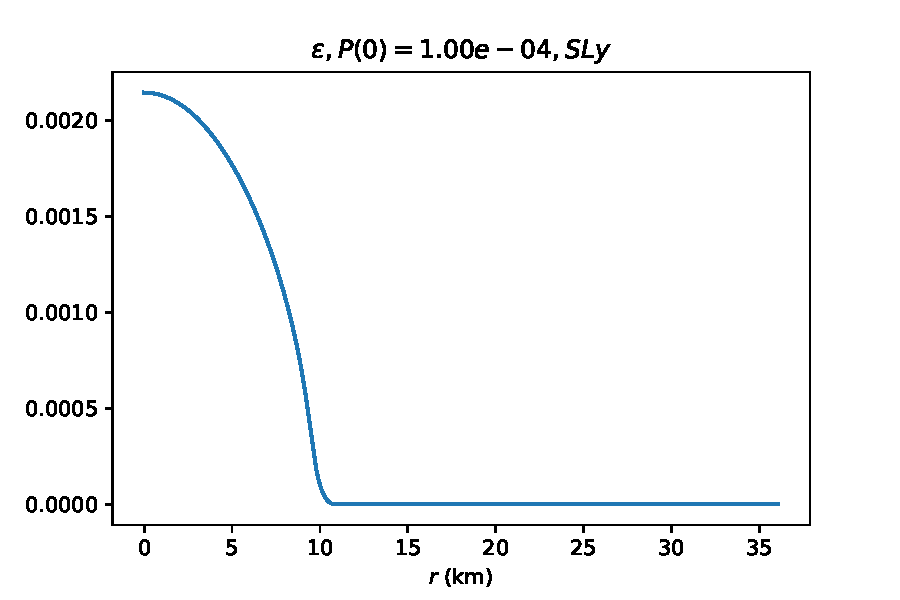
\includegraphics[width = \textwidth]{../paper/images/tov/SLy_rho,p00.0001.pdf}
            \end{subfigure}
            \caption[]{Example static solution for $P_0 = \SI{e-4}{}$ for an EoS called ``SLy.''}
        \end{figure}
    \end{frame}

    \begin{frame}{Static Solutions: $M(R)$ and $M(P_0)$ diagrams}
        \pause
        Use static solutions to make predictions using an EoS: \pause
        \begin{enumerate}
            \item Create static solutions for a range of $P_0$ values: \pause $P_0 \in [\SI{e-6}{}, \SI{e-1}{}].$\pause
            \item Find and store the mass $M$ and radius $R$ for each value of $P_0$.\pause
            \item Create $M(R)$ and $M(P_0)$ curves\pause
        \end{enumerate}

        \begin{figure}[h!]
            \centering
            \begin{subfigure}{.5\textwidth}
                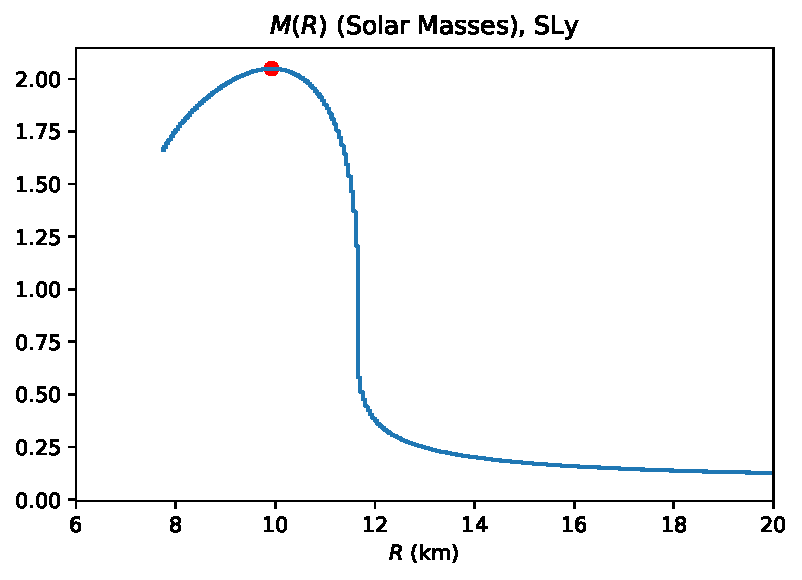
\includegraphics[width = \textwidth]{../paper/images/tov/r_analysis,SLy.pdf}
            \end{subfigure}%
            \begin{subfigure}{.5\textwidth}
                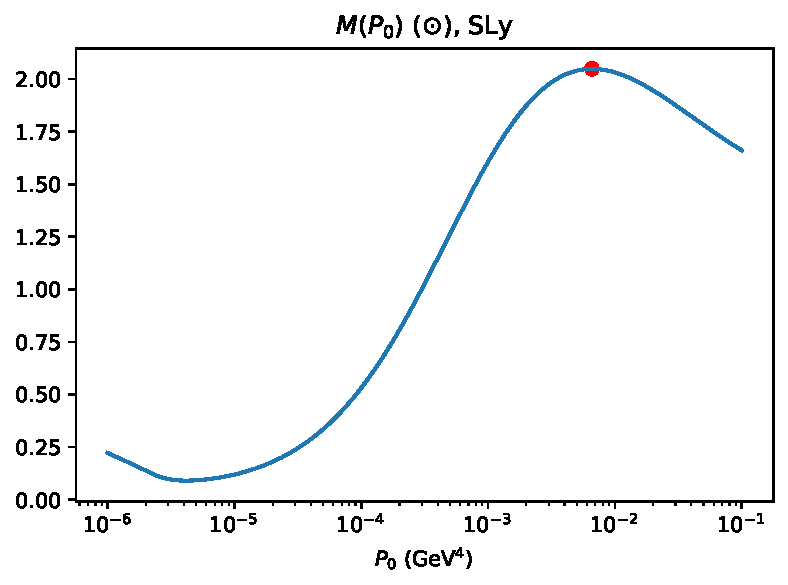
\includegraphics[width = \textwidth]{../paper/images/tov/p0_analysis,SLy.pdf}
            \end{subfigure}
            \caption[]{Example curves for EoS ``SLy.'' $\SI{1}{\odot} = \SI{1.989e+30}{kg}$ (solar mass)}
        \end{figure}
    \end{frame}

    \begin{frame}{Critical Values of $P$, $R$, and $M$}
        \vspace{-10pt}
        \begin{figure}[h!]
            \centering
            \begin{subfigure}{.5\textwidth}
                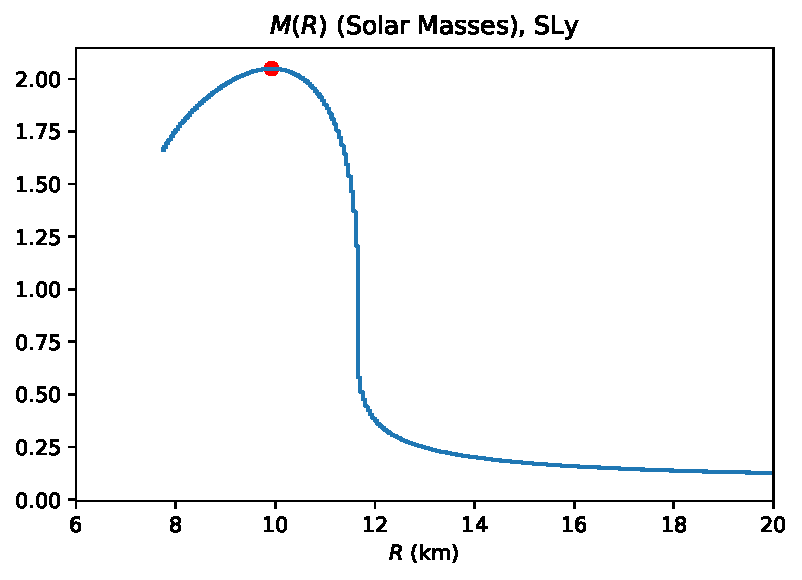
\includegraphics[width = \textwidth]{../paper/images/tov/r_analysis,SLy.pdf}
            \end{subfigure}%
            \begin{subfigure}{.5\textwidth}
                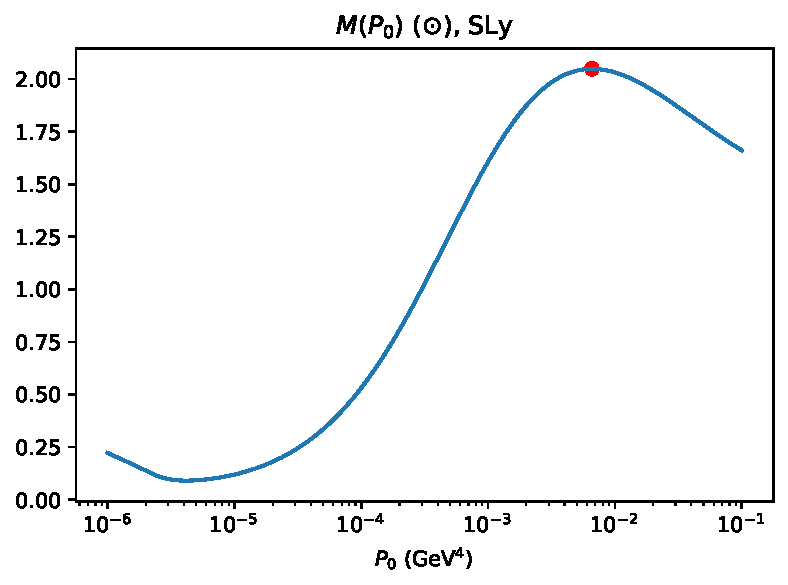
\includegraphics[width = \textwidth]{../paper/images/tov/p0_analysis,SLy.pdf}
            \end{subfigure}
        \end{figure} \pause
        Three important values: \pause \textit{critical pressure, critical mass,} and \textit{critical radius}. \pause 
        \begin{itemize}
            \item Determined by ``peaks'' of graph \pause
            \item Maximum mass and radius predicted by EoS \pause
            \item Largest ``stable'' pressure \pause
            \item For SLy, $M_\text{max} = \SI{2.05}{\odot}$, $R_\text{max} = \SI{9.93}{km}$, and $P_\text{crit} = \SI{6.59e-3}{}$.
        \end{itemize}

    \end{frame}

    % \begin{frame}{Quantum Hadrodynamics}
    %     \pause
    %     A theory of the quantum mechanical, interparticle interactions within a neutron star. \pause
    %     \begin{itemize}
    %         \item Formulation of nuclear interactions between \textit{baryons} by the exchange of \textit{mesons} \pause \begin{itemize}
    %             \item \textit{baryons} are particles containing three quarks (e.g. protons, neutrons) \pause
    %             \item \textit{mesons} are quark/anti-quark pairs\pause
    %         \end{itemize}
    %         \item Requires experimental input for constraint; \pause implemented using \textit{coupling constants} \pause \begin{itemize}
    %             \item Multiple \textit{parameter sets} have been developed by fitting observed nuclear properties of nuclear matter \pause
    %         \end{itemize}
    %         \item Considered quite complicated to solve\pause ; we introduce some simplifications in the QHD-I model
    %     \end{itemize}
    % \end{frame}

    \begin{frame}{Quantum Hadrodynamics}
        \pause A theory of the interactions between the subatomic particles in the core of a neutron star
        \pause
        \begin{itemize}
            \item The protons and neutrons influence one another (e.g. apply forces); \pause mediated by exchanging a particle \pause (called a \textit{meson}) \pause
            \item Describe these interactions mathematically; \pause the Lagrangian $\Lag$ \pause
        \end{itemize}
        Model requires input from actual experiments \pause
        \begin{itemize}
            \item Extreme conditions in core of a neutron star are not reproducible \pause (e.g. pressures are too high, etc.) \pause
        \end{itemize}
        Equations of Quantum Hadrodynamics are considered very difficult to solve; \pause introduce simplifications in the QHD-I model
    \end{frame}

    \begin{frame}{Quantum Hadrodynamics I (QHD-I)}
        We form the \textit{Lagrangian} (encodes information about the energy in the system): \pause
        \begin{align*}
            \Lag & = \bar{\psi} \bqty{\gamma_\mu(i\p^\mu -g_v V^\mu) - (M-g_\phi\phi)} \psi \nonumber\\
            & \quad + \frac{1}{2} \pqty{\p_\mu \phi \p^\mu \phi - m_\phi^2 \phi^2} - \frac{1}{4} V_{\mu\nu}V^{\mu\nu} + \frac{1}{2} m_v^2 V_\mu V^\mu,
        \end{align*}\pause
        where
        \begin{itemize}
            \item Nucleons (protons and neutrons) $\psi$ \pause
            \item Mesons: $\phi$ and $V$ \pause
            \item Constants from experiment: $g_v$ and $g_\phi$ \pause
        \end{itemize}
        From $\Lag$, we can determine $\epsilon$ and $P$, the EoS we desire.
    \end{frame}

    \begin{frame}{RMF Simplifications}
        We introduce the \textit{Relativistic Mean Field} (RMF) simplifications. \pause We treat the interactions (exchange of mesons) as their average values: \pause
        \[\phi \to \expval{\phi} = \phi_0, \quad V_\mu \to \expval{V_\mu} = V_0,\]
        where $\phi_0$ and $V_0$ are constants. \pause This allows us to simplify $\Lag$ considerably: \pause
        \begin{align*}
            \Lag_\text{RMF} = \bar\psi \bqty{i\gamma_\mu\p^\mu - g_v \gamma_0 V_0 - (M-g_s\phi_0)} \psi - \frac{1}{2} m_s^2 \phi_0^2 + \frac{1}{2} m_\omega^2 V_0^2,
        \end{align*} \pause
        Determining $\phi_0$, $V_0$, $\epsilon$, and $P$: \pause $\quad\varphi_\alpha \in \Bqty{\phi_0, V_0, \psi}$
        \[\p_\nu\qty(\pdv{\Lag}{(\p_\nu \varphi_\alpha)}) - \pdv{\Lag}{\varphi_\alpha} = 0, \quad
        T^{\mu\nu} = \pdv{\Lag}{(\p_\mu \varphi_\alpha)}\p^\nu \varphi_\alpha - \Lag \eta^{\mu\nu}.\] \pause
        $$\epsilon = \expval{T^{00}}, \quad P = \expval{T^{ii}}$$
    \end{frame}

    \begin{frame}{Resulting Equations}
        From above, we obtain the following equations: \pause
        \begin{align*}
            \phi_0 &= \frac{g_\phi}{m_\phi^2} \frac{1}{\pi^2} \int_0^{k_f} \dd{k} \frac{(M-g_\phi \phi_0) k^2 }{\sqrt{k^2 + (M-g_\phi \phi_0)}},  \\
            V_0 &= \frac{g_v}{m_v^2} \frac{k_f^3}{3\pi^2}, \\
            \epsilon & = \frac{1}{2} m_\phi^2 \phi_0^2 + \frac{1}{2} m_v^2 V_0^2 + \frac{1}{\pi^2} \int_0^{k_f} \dd{k} k^2 \sqrt{k^2 + m^{*2}},\\
            P & = -\frac{1}{2} m_\phi^2 \phi_0^2 + \frac{1}{2} m_v^2 V_0^2 + \frac{1}{3} \pqty{\frac{1}{\pi^2} \int_0^{k_f} \dd{k}\frac{k^4}{\sqrt{k^2 + m^{*2}}}}.
        \end{align*}
        where $m^* = (M-g_\phi \phi)$, the \textit{reduced mass}. 
    \end{frame}

    \begin{frame}{Resulting Equations}
        From above, we obtain the following equations:
        \begin{align*}
            \phi_0 = \phi_0(k_f, \phi_0), &\quad  
            V_0 = V_0(k_f), \\
            \epsilon = \epsilon(k_f,\phi_0,V_0), &\quad
            P  = P(k_f,\phi_0,V_0).
        \end{align*}
        \pause Goal: \pause create a list of values that show us $\epsilon(P)$; \pause each value of $k_f$ gives us a different $\epsilon$ and $P$. \pause

        \medskip
        To produce the EoS: \pause (repeat the following) \pause
        \begin{itemize}
            \item Choose a $k_f$ value \pause
            \item calculate $\phi_0$ and $V_0$\pause; use \textit{rootfinding} for $\phi_0$\pause
            \item Using those values, calculate $P$ and $\epsilon$ and store in a table
        \end{itemize}
    \end{frame}

    % \begin{frame}{Producing the Equation of State}

    %     Steps: \pause
    %         \begin{align*}
    %             \phi_0 = f(k_f, \pause \phi_0), \pause \quad
    %             V_0 = \frac{g_v}{m_v^2} \frac{k_f^3}{3\pi^2} 
    %         \end{align*}
    %         \item Using those values, calculate $P$ and $\epsilon$ and store in a table
    %     \end{itemize}
    % \end{frame}
    
    \begin{frame}{$M(R)$ and $M(P_0)$ Curves for QHD-I}
        We use the tabulated values of $P$ and $\epsilon$ to solve the TOV equations: \pause
        \begin{figure}[h!]
            \centering
            \begin{subfigure}{.5\textwidth}
                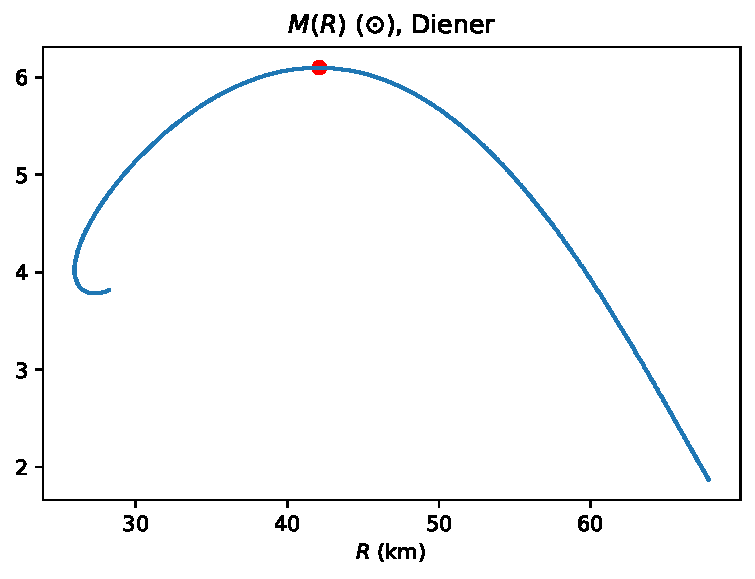
\includegraphics[width = \textwidth]{../paper/images/qhd1/r_analysis.pdf}
            \end{subfigure}%
            \begin{subfigure}{.5\textwidth}
                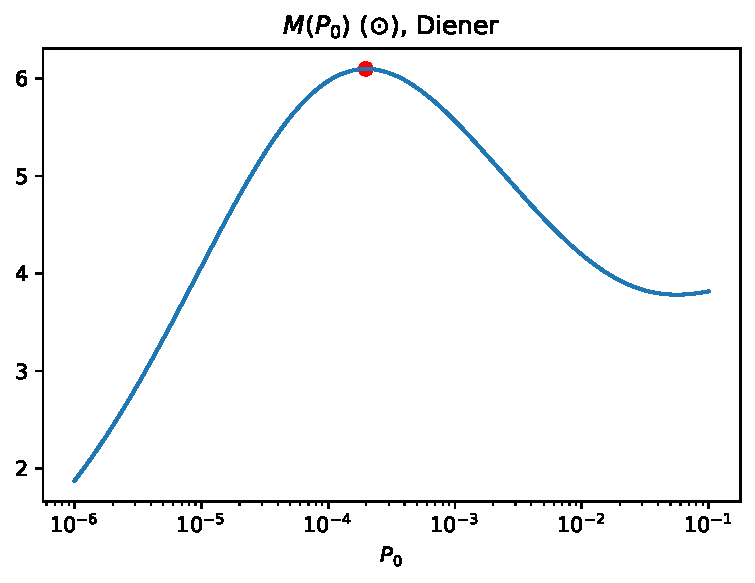
\includegraphics[width = \textwidth]{../paper/images/qhd1/p0_analysis.pdf}
            \end{subfigure}
            \caption[]{$M(R)$ and $M(P_0)$ curves for QHD-I EoS.}
        \end{figure}\pause
        \vspace{-3pt}
        These curves give \[M_\text{max} = \SI{6.1}{\odot}, \quad R_\text{max} = \SI{42.1}{km}, \quad P_\text{crit} = \SI{1.98e-4}{}.\]
    \end{frame}

    \begin{frame}{Conclusion}
        \begin{itemize}
            \item An equation of state is a relationship between energy density and pressure within a neutron star \pause
            \item We use the TOV equations to predict the maximum mass and radius that a given EoS will produce \pause
            \item We use the QHD-I parameter set and RMF simplifications to solve a system of equations and generate an equation of state
        \end{itemize}
    \end{frame}

    \begin{frame}{Thanks}
        \begin{itemize}
            \item Prof. Ben Kain \pause
            \item Holy Cross Physics Department \pause
            \item My family \pause
            \item Special thanks: Prof. Perry and the AV team
        \end{itemize}
    \end{frame}
\end{document}
